\subsection{Introducción a GNU Radio}

\begin{frame}{}

\pgfdeclareimage[width=\paperwidth,height=\paperheight]{bg}{imagenes/fondo_lab}
\setbeamertemplate{background}{\pgfuseimage{bg}}

\bfseries{\textrm{\Large \\Introducción a GNU Radio}}
\raggedright
\end{frame}



\begin{frame}
  
\pgfdeclareimage[width=\paperwidth,height=\paperheight]{bg}{imagenes/fondo3}
\setbeamertemplate{background}{\pgfuseimage{bg}}
  
  \frametitle{¿Qué es GNU Radio\index{GNU RADIO}?}

  
  Es una herramienta de desarrollo libre y abierta que provee bloques de procesamiento de señal para implementar sistemas de radio definido por software. Puede utilizarse con hardware de RF para crear radios definidos por
software o sin hardware para crear un ambiente de simulación. Es utilizada
extensivamente en ambientes académicos, aficionados y comerciales para dar
soporte a la investigación en comunicaciones inalámbricas y en sistemas de
radio en el mundo.
\end{frame}



\begin{frame}{Aplicaciones\index{Aplicaciones}}
  \begin{figure}[H]
  \centering
  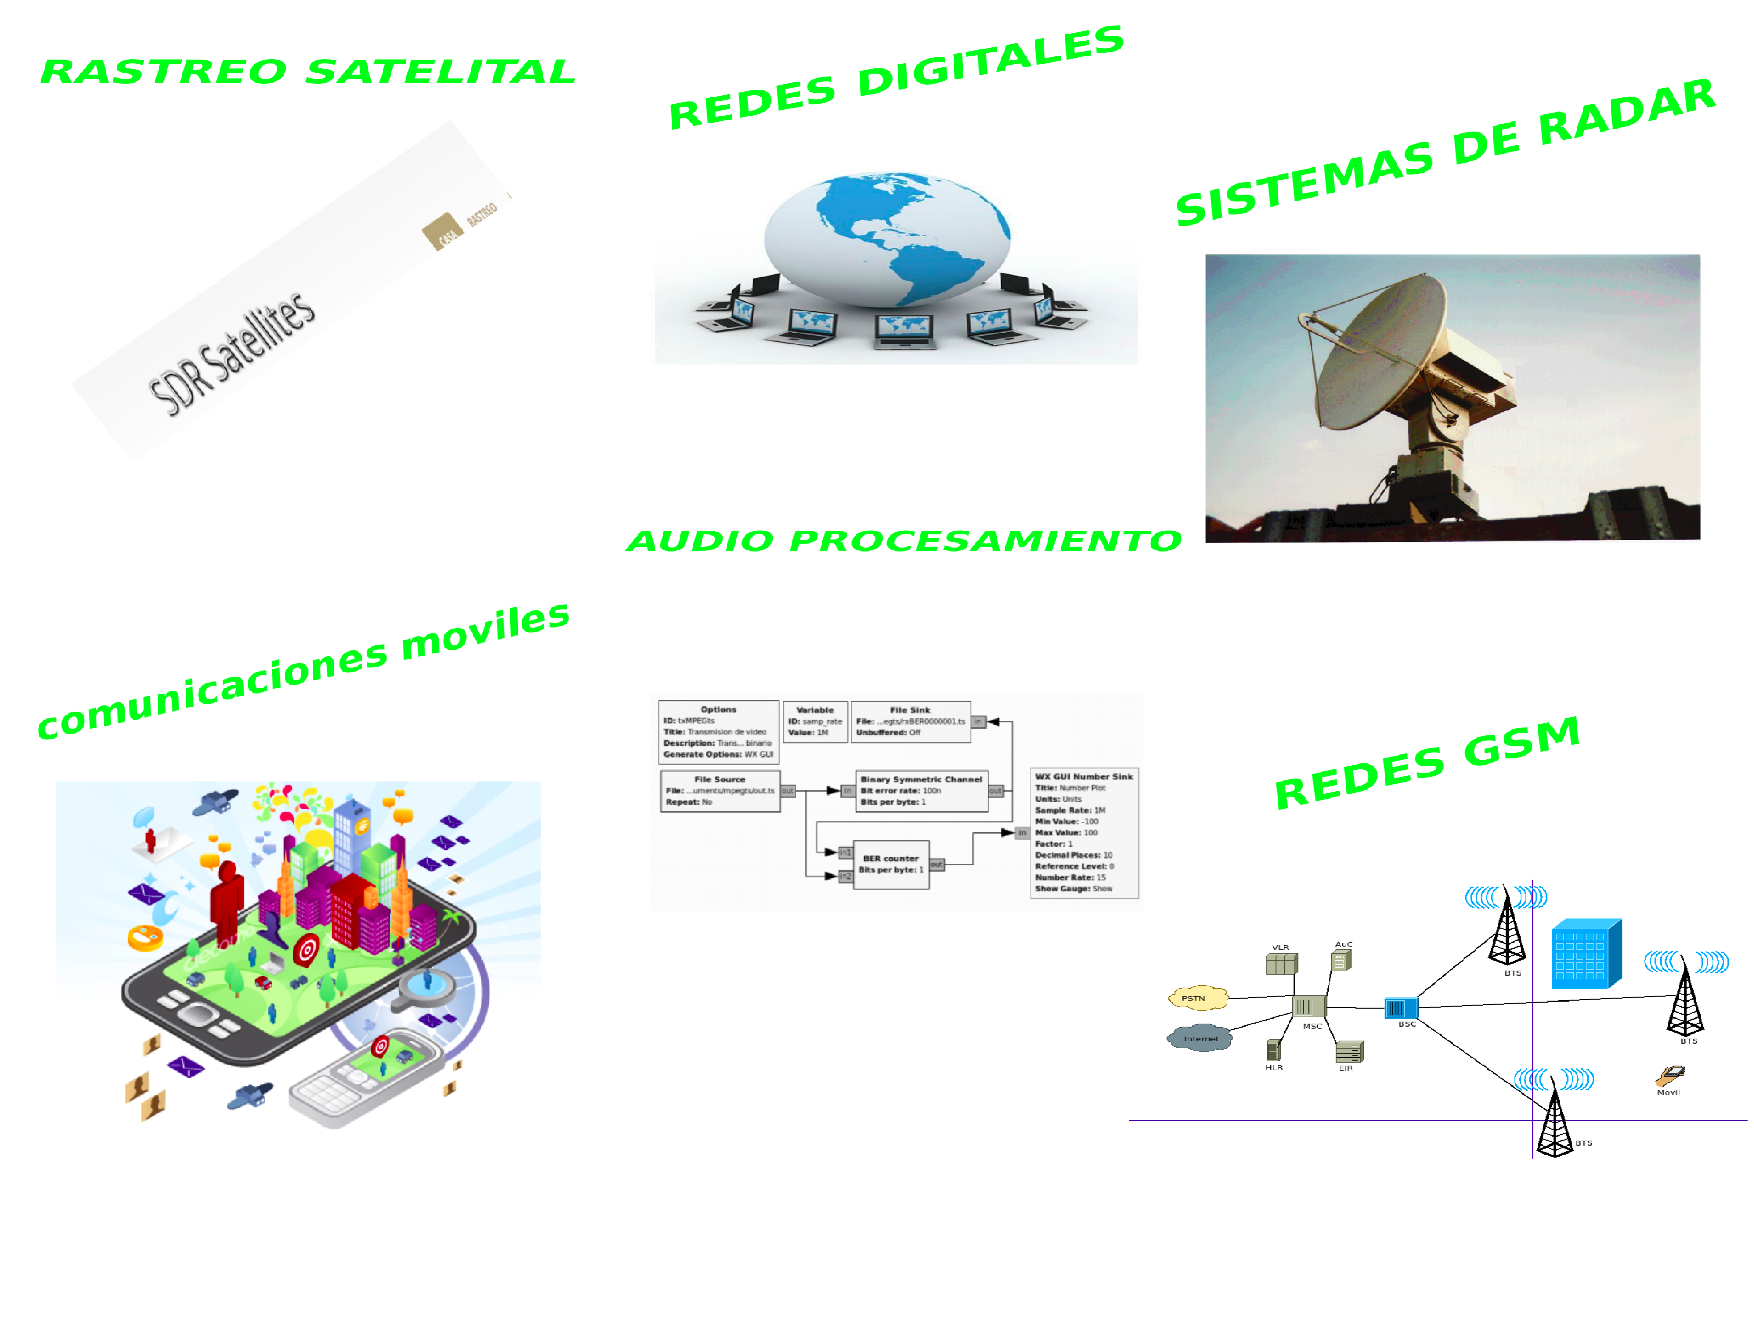
\includegraphics[width=0.9\textwidth]{parte1/intro/pdf/intro.pdf}
  \end{figure}
  
  
\end{frame}



\begin{frame}{Instalación de GNU Radio en Linux}
{Para instalar GNU Radio se deben seguir los siguientes pasos:}
\begin{enumerate}[1.]
\item Ingresar a la ventana de órdenes (o terminal) del sistema de su equipo.
\item Estando conectado a internet, escriba dentro del terminal:

  \begin{block}{}
  \texttt{
    sudo apt-get install gnuradio}
  \end{block}

\item Si su dispositivo tiene contrase\~na, debe ingresarla, al ser solicitada y oprimir \keys{\return}. 
\item Luego se deben aceptar los términos de la instalación oprimiendo la letra \keys{s} seguido de \keys{\return}. 
\item Una forma de verificar la correcta instalación es volviendo a ingresar el comando indicado en el punto 2, y si aparece un mensaje anunciando que GNU Radio ya está en su versión más reciente, su instalación fue correcta.
\end{enumerate}
\end{frame}
%----------------------------

\begin{frame}{Paquetes\index{Paquetes}}
Con el objetivo de clonar el repositorio y obtener los ejemplos de GNU Radio en nuestro ordenador se deben instalar los siguientes paquetes: 
  \begin{itemize}
  \item {BUILD-ESSENTIAL\\}
    \begin{itemize}
    \item
    {Build essential es un paquete que contiene herramientas necesarias
    para la creación, compilación e instalación de programas.}
    \end{itemize}
  \item {CMAKE\\}
  {Es un sistema de construcción de código abierto multiplataforma. Se trata de  un conjunto de herramientas diseñadas para construir, testear y empaquetar software. Se utiliza para controlar el proceso de compilación de software utilizando una plataforma sencilla y unos archivos de configuración
independientes del compilador.}
  \end{itemize}
\end{frame}
%-------------------------------

\begin{frame}{Paquetes}
  \begin{itemize}
  \item {GIT\\}
  \begin{itemize}
    \item
    {Este paquete contiene una Git; es un sistema de control de versiones distribuidas de código abierto desarrollado originalmente por Linux Torvalds para apoyar el desarrollo del kernel de Linux.}
    \item
    {El control de versiones es un sistema que registra los cambios realizados sobre un archivo o conjunto de archivos a lo largo del tiempo, de modo que se puedan recuperar versiones específicas más adelante.}
    \end{itemize}
  \item {LIBBOOST-ALL-DEV\\}
  {Es una biblioteca de software libre y revisión por partes preparadas para extender las capacidades del lenguaje de programación; permite ser utilizada en cualquier tipo de proyectos.}
  \end{itemize}
\end{frame}

%++++++++++++++++++++

\begin{frame}{Paquetes\index{Paquetes}}
  \begin{itemize}
  \item {LIBCPPUNIT-DEV\\}
  \begin{itemize}
    \item
    {Biblioteca de pruebas unitarias para C++.}
    \item
    {Una prueba unitaria es una forma de comprobar el correcto
funcionamiento de una unidad de código. Por ejemplo, en diseño
estructurado o en diseño funcional, una función o un procedimiento,
en diseño orientado a objetos una clase. Esto sirve para asegurar que
cada unidad funcione correcta y eficientemente por separado.}
    \end{itemize}
  \item {DOXYGEN\\}
  {Es una herramienta para generar documentación a partir de código fuente. Es un sistema de documentación para C++, C, Java, Python. Es necesario solo si se desea generar referencias a documentación externa de la que no tiene las fuentes.}
  \end{itemize}
\end{frame}

%+++++++++++++++++++

\begin{frame}{Instalación de paquetes}
\begin{enumerate}[1.]
\item La instalación de cada uno se los paquetes anteriormente mencionados se realiza colocando en la ventana de terminal, las siguientes órdenes:
\end{enumerate}

  \begin{block}{}
  \texttt{
  \ \ \ sudo apt-get install build-essential
    \begin{itemize}
      \item[] sudo apt-get install cmake
      \item[] sudo apt-get install git
      \item[] sudo apt-get install libboost-all-dev
      \item[] sudo apt-get install libcppunit-dev
      \item[] sudo apt-get install doxygen
    \end{itemize}}
  \end{block}


\end{frame}

%++++++++++++++++++++


\begin{frame}{Clonar repositorio\index{Clonar Repositorio}}
El código fuente de los ejemplos está almacenado en github, por lo tanto para clonar el repositorio se debe realizar lo siguiente:
\begin{itemize}
\item Abrir la ventana de órdenes o terminal.
\item Después se debe ingresar la siguiente orden para clonar el directorio git:

\begin{block}{}
  \texttt{
    git clone https://github.com/gnuradio/gr-tutorial}
  \end{block}

\item Una vez clonado el directorio, , en el PC empleado se deben ver exactamente los mismos archivos y carpetas que los del repositorio github.
\end{itemize}
\end{frame}

%+++++++++++++++++++

\begin{frame}{Instalación de módulos\index{Modulos}}
\begin{itemize}
\item Luego de haber clonado el repositorio, debemos buscar la carpeta \textbf{“gr-tutorial”} e ingresar a ella desde el terminal, para ello se digitan los siguientes mandos:

  \begin{block}{}
  \texttt{
  \ \ \ ls
    \begin{itemize}
      \item[] cd gr-tutorial
    \end{itemize}}
  \end{block}

Es importante mencionar que al escribir el primer comando se podrán observar la diferentes carpetas que se encuentran en el dispositivo, por lo tanto \textbf{“gr-tutorial”} debe aparecer entre las opciones para poder cambiar de directorio. 
\end{itemize}
\end{frame}

%+++++++++++++++

\begin{frame}{Instalación de módulos\index{Modulos}}
\begin{itemize}
\item Estando dentro de la carpeta, desde la terminal, se deben escribir los siguientes mandos, con la finalidad de instalar las soluciones o módulos:

  \begin{block}{}
  \texttt{
  \ \ \ mkdir build
    \begin{itemize}
      \item[] cd build
      \item[] cmake ..
      \item[] make -j8
      \item[] sudo make install
      \item[]sudo ldconfig
    \end{itemize}}
  \end{block}

\end{itemize}
\end{frame}
